\documentclass{standalone}
\usepackage{amsmath,amssymb,amsthm}
%\usepackage[usenames,dvipsnames,table]{xcolor}
%\usepackage{graphicx} 										% Graphics
\usepackage{tikz} \usetikzlibrary{calc,arrows.meta,intersections,patterns} 	% Figure
\usepackage{pgfplots}

%% !TEX root = ThesisManuscript_SJ.tex
%%
%%
%%	COLORS
%%_______________________________________________
\definecolor{MyBlue}{RGB}{0,120,155}
\definecolor{MyDarkBlue}{rgb}{0, 0.25, 0.45}
\definecolor{MyBrown}{rgb}{0.28, 0.20, 0.20}
\definecolor{MyOrange}{RGB}{255,80,30}
\definecolor{MyOldOrange}{rgb}{0.75, 0.25, 0.0}
\definecolor{MyRed}{RGB}{200,0,0}
\definecolor{MyGray}{RGB}{200,200,200}
\definecolor{MyGreen}{rgb}{0.33, 0.5, 0.18}
\definecolor{MyDarkGreen}{rgb}{0.15, 0.25, 0.18}
\definecolor{MyTurquoise}{rgb}{0, 0.4, 0.4}
\definecolor{MyViolet}{rgb}{0.44, 0.16, 0.39}
\definecolor{MyYellow}{rgb}{1, 0.65, 0}

\begin{document}
\centering

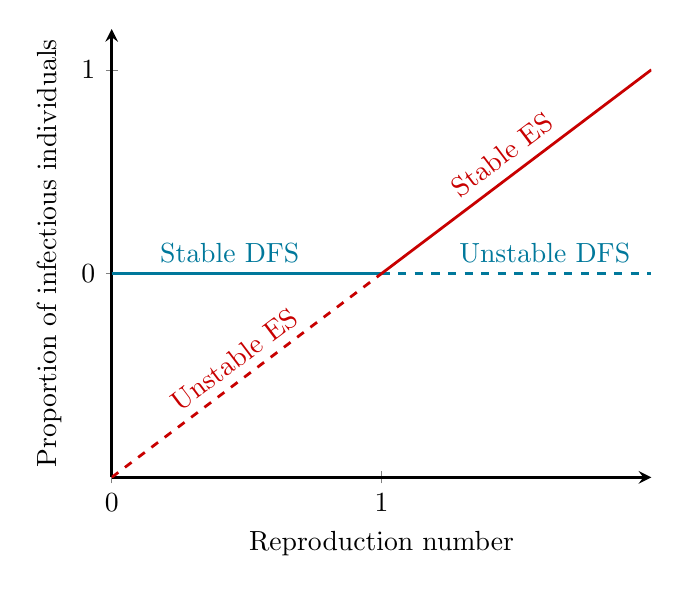
\begin{tikzpicture}[line width=1pt]
\begin{axis}[
    axis lines = left,
    xlabel = {Reproduction number},
    ylabel = {Proportion of infectious individuals},
    xtick={0,1},
    ytick={0,1},
    ymax=1.2,
    line width = {1pt},
%    xmajorgrids=true,
%    ymajorgrids=true,
]
% Stable DFS
\addplot [
    domain=0:1, 
    samples=2, 
    color = MyBlue,
    line width = 1pt,
]
{0};
%\addlegendentry{\textcolor{MyBlue}{Stable DFS}}
% Unstable DFS
\addplot [
    domain=1:2, 
    samples=2, 
    color = MyBlue,
    line width = 1pt,
    style = dashed,
]
{0};
%\addlegendentry{\textcolor{MyBlue}{Unstable DFS}}
% Stable ES
\addplot [
    domain=1:2, 
    samples=2, 
    line width = 1pt,
    color = MyRed,
    ]
    {x - 1};
%\addlegendentry{\textcolor{MyRed}{Stable ES}}
% Unstable ES
\addplot [
    domain=0:1, 
    samples=2, 
    line width = 1pt,
    color = MyRed,
    style = dashed,
    ]
    {x - 1};
%\addlegendentry{\textcolor{MyRed}{Unstable ES}}
%
\end{axis}
        	\draw (1.5,2.6) node (SDFS)[above, color=MyBlue] {Stable DFS};
        	\draw (5.5,2.6) node (UDFS)[above, color=MyBlue] {Unstable DFS};
	\draw (1.7,1.3) node (UES)[above, rotate=37, color=MyRed] {Unstable ES};
	\draw (5.1,3.9) node (SES)[above, rotate=37, color=MyRed] {Stable ES};
\end{tikzpicture}

\end{document}

